% Klassifiziert den Dokumenten-Typ
% Doku: http://exp1.fkp.physik.tu-darmstadt.de/tuddesign/
% Farben: http://www.tu-darmstadt.de/media/medien_stabsstelle_km/services/medien_cd/das_bild_der_tu_darmstadt.pdf
%  bigchapter: Chapter haben doppelte Schriftgröße
%  linedtoc: Linien im Inhaltsverzeichnis wie bei Überschriften
%  colorbacktitle: Der Dokumenten-Titel wird mir der Accentfarbe hinterlegt
\documentclass[bigchapter,colorback,accentcolor=tud4b,linedtoc,11pt]{tudreport}

% Input Dokument hat das Encoding UTF-8
\usepackage[utf8]{inputenc}
% Wichtiges Paket für Links und verlinktes Inhaltsverzeichnis
\usepackage[ngerman]{hyperref}
% Paket für Fußnoten
\usepackage[stable]{footmisc}
% Paket für amsmath (aligned mathe formeln)
\usepackage{amsmath}
% Paket für Bibliotheks-Verzeichnis, square: Verwende eckige statt runde klammern
% \usepackage[square]{natbib}
% Paket zum Plotten von Datensätzen
\usepackage{pgfplots}
\usepgfplotslibrary{patchplots}


\pgfkeys{%
  /pgfplots/seperators/.style={%
    /pgf/number format/use comma
  }
}

% Anhänge für Original-Messdaten
\usepackage{fancyvrb}

% redefine \VerbatimInput
\RecustomVerbatimCommand{\VerbatimInput}{VerbatimInput}%
{fontsize=\footnotesize,
 %
 frame=lines,  % top and bottom rule only
 framesep=2em, % separation between frame and text
 fontsize=\scriptsize,
 %
 labelposition=topline,
 %
 commandchars=\|\(\), % escape character and argument delimiters for
                      % commands within the verbatim
 commentchar=*        % comment character
}

% Polar Plots
\usetikzlibrary{pgfplots.polar}
% Verwende deutsche Bezeichner für Inhaltsverzeichnis, ... (ngerman = New German: neue Rechtschreibung)
\usepackage{ngerman}
% Deutsche Zahlen (entfernt z.B. das Leerzeichen nach einem Dezimal-Komma)
\usepackage{ziffer} 

\usepackage[verbose]{placeins}

%wegen Grafikverschiebung hinzugefügt
\usepackage{float}

%\usepackage{graphicx}
%\usepackage{caption}
\usepackage{subcaption} %Für subfigures

% PDF-Optionen
\hypersetup{%
  pdftitle={TU Darmstadt \- Physikalisches Praktikum für Fortgeschrittene},
  pdfauthor={Esra Bauer und Sören Link},
  pdfsubject={Versuch 1.1},
  pdfview=FitH,
}
% Nummeriere formeln in Subsections einzeln
% Kleines makro zur assymetrischen Fehlerangabe

% Entspricht-Zeichen
\usepackage{scalerel}

\newcommand\equalhat{%
\let\savearraystretch\arraystretch
\renewcommand\arraystretch{0.3}
\begin{array}{c}
\stretchto{
    \scalerel*[\widthof{=}]{\wedge}
    {\rule{1ex}{3ex}}%
}{0.5ex}\\ 
=%
\end{array}
\let\arraystretch\savearraystretch
}
%BEGINN TITELSEITE

\title{Magnetfeldmessung}

\subtitle{Esra Bauer  \\Sören Link}

\subsubtitle{Betreuer: Thore Bahlo \hfill Versuchsdatum: 28. Januar 2015}

\author{Esra Bauer, Sören Link}

%\settitlepicture{img/title.jpg}

\institution{Physikalisches Praktikum \\für Fortgeschrittene \\ Versuch 1.1}

\date{\today}


%ENDE TITELSEITE

\begin{document}
%ANFANG DOKUMENT

%Titelseite einfügen
\maketitle

%Inhaltsverzeichnis einfügen
\tableofcontents

%ANFANG INHALT

\chapter{Einleitung}

In diesem Versuch geht es um die Vermessung von Elektromagneten, wie sie in Teilchenbeschleunigeranlagen eingesetzt werden. In diesem Gebiet ist oft eine hohe Genaugkeit für die Fokussierung und Richtung des Teilchenstrahls erforderlich, weshalb die Magnete präzise gefertigt und montiert werden müssen. Anhand  des Praktikumsversuchs wird aufgezeigt, wie man die charakteristischen Größen der jeweiligen Magnete, also die magnetische Flussdichte eines Dipolmagneten und den Feldgradienten eines Quadrupolmagneten quantitativ untersuchen kann und somit z.B. Rückschlüsse auf die Qualität des Magneten oder dessen Ausrichtung treffen kann.

\chapter{Grundlagen}
\section{Hall-Effekt}
Der große Teil der Messungen in diesem Versuch wird mit einer Hall-Sonde durchgeführt, deren Funktionsweise auf dem nach Edwin Hall benannten Hall-Effekt beruht. Dieser beschreibt das Entstehen einer Spannung in einem stromdurchflossenen Leiter, der sich in äußeren Magnetfeld befindet.

Diese Spannung lässt sich aus der Tatsache ableiten, dass Strom durch bewegte Elektronen hervorgerufen wird. Da Elektronen geladene Teilchen sind, wirkt bei der Bewegung im Magnetfeld die Lorenzkraft $$\vec{F_L} = q \cdot \vec{v} \times \vec{B}$$

Beschränkt man sich auf die Messung der Magnetfeldkomponente senkrecht zur Ausrichtung des Leiters bzw.\ der Hall-Sonde, so lässt sich diese Gleichung o.b.d.A. schreiben als
$$\vec{F_L} = q \cdot v \cdot \vec{e_x} \times B \cdot \vec{e_z}$$
$$\vec{F_L} = q \cdot v  \cdot B \cdot \vec{e_y}$$

Diese Kraft auf die bewegten Elektronen führt zu einer inhomogenen Ladungsverteilung der Elektronen , wodurch ein Elektrisches Feld aufgebaut wird. Dieses übt ebenfalls eine Kraft 
$$\vec{F_E}=q \cdot \vec{E}$$
auf die Elektronen aus, welche der Lorenzraft entgegengerichtet ist. Bereits nach sehr kurzer Zeit stellt sich somit ein Gleichgewichtszustand ein:
$$q \cdot \vec{E} = q \cdot v  \cdot B \cdot \vec{e_y}$$
Geht man von einem homogenen elektrischen Feld in einem Leiter der Breite b entlang der y-Richung aus, so lässt sich das Feld schreiben als 
$$\vec{E} = \frac{U_H}{b}\cdot \vec{e_y}$$
Einsetzen in die Gleichgewichtsgleichung und Auflösen nach $U_H$ ergibt
$$U_H = b \cdot v \cdot B$$

Leider ist die Geschwindigkeit $v$ der Elektronen in der Regel nicht direkt messbar, weswegen diese durch die angelegten Stromstärke 
$$I= n\cdot q \cdot b \cdot d \cdot v$$
mit den Leiterspezifischen Größen für die Dicke $d$ und der Ladungsträgerdichte $n$, ausgedrückt werden muss.

Fasst man zusätzlich noch alle Sondenspezifischen größen in der Hall-Konstanten $R_H = \frac{1}{n\cdot q}$ zusammen, erhält man die Formel

$$U_H = R_H \frac{I\cdot B}{d}$$

\section{Elektromagnetismus}
\subsection{Ferromagnetismus}

Ferromagnetische Stoffe sind im inneren aus sogenannten Weißschen Bezirken aufgebaut, welche aus parlell angeordneten magnetischen Dipolen, sogenannten Elementarmagneten bestehen.
Diese Bezirke kommen dadurch Zustande, dass die zuerst zufällig ausgerichteten Elementarmagnete mit benachtbarten Elementarmagneten wechselwirken und sich paralell zueinander ausrichten. Dadurch wird deren magnetische Kraft verstärkt und die Wechselwirkungsreichweite steigt an, es richten sich immer mehr benachtbarte Elementarmagnete gleich aus. Durch den statistischen Charakter der ursprünglichen Ausrichtung der Elementarmagnete, sind die Magnetisierungsrichtungen zweier so herangewachsener benachtbarter Bezirke allerdings in der Regel nicht gleich ausgerichtet.

Wird jedoch jetzt ein äußeres Magnetfeld angelegt, können zum Magnetfeld ähnlich ausgerichtete Bezirke "`umklappen"', wodurch die Anzahl der paralell zum äußeren Magnetfeld ausgerichteten Bezirke erhöht wird, was wiederrum das angelegte Magnetfeld verstärkt. Je stärke das von außen angelegte Magnetfeld ist, desto mehr Weißsche Bezirke werden zur änderung ihrer Magnetisierungsrichtung gezwungen, und desto stärker wird das äußere Magnetfeld verstärkt. Ab einer Gewissen äußeren Magnetfeldstärke sind allerdings nahezu alle Bezirke paralell ausgerichtet und es wird eine Sättigung der Verstärkung erreicht. Bei den meisten Ferromagneten geschieht dies ab einer Magnetfeldstärke von etwa $1T$.

Wird nach einmaliger Magnetisierung das äußere Magnetfeld wieder abgeschaltet, so wird die paralelle Ausrichtung der Weißschen Bezirke im Ferromagneten durch thermische Prozesse nur zum Teil weider aufgehoben, es bleibt einer gewisse Restmagnetisierung des Ferromagneten bestehen. Dieser Effekt wird Hysterese genannt.

\begin{figure}[H]
\centering
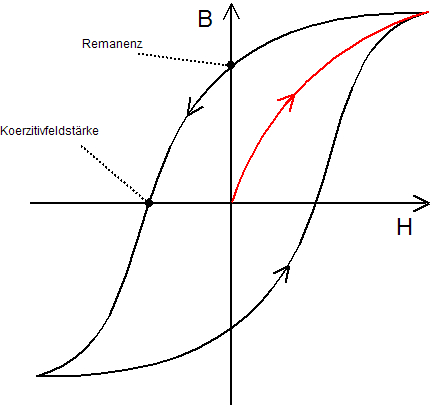
\includegraphics[width=80mm]{img/hysterese.png}
\caption{Typische Hysteresekurve eines Ferromagneten. Der rote Pfeil beschreibt die erstmalige Magnetisierung des Materials. Als Remanz wird die verbleibende Magnetisierung bezeichnet, die nach Abschalten des äußeren Feldes übrig bleibt. Die Koerzitivfäldstärke beschreibt dagegen die Feldstärke die entgegen der ursprügnlichen Richtung angegelgt werden muss, um die Magnetisierung des Ferromagneten aufzuheben.\cite{hysterese}}
\end{figure}

\subsection{Dipolmagnete}

Dipolmagnete werden häufig in der Beschleunigerphysik zur Umlenkung von hochenergetischen Teilchenstrahlen verwendet. Sie bestehen aus einem magnetischen Nord- und einem Südpol, zwischen welchem im Idealfall ein homogenes Magnetfeld besteht. Passiert ein Teilchenstrahl dieses Magnetfeld, so wird er auf Grund der Lorenzkraft $\vec{F_L} = q \cdot \vec{v} \times \vec{B}$ senkrecht zur Magnetfeld und seiner Bewegungsrechtung abgelenkt. Anstatt eines Dipolmagneten kann man zwar theoretisch auch ein elektrisches Feld, z.B. das Feld zwischen den Platten eines Plattenkondensators, benutzen, allerdings skaliert die auf einen Teilchenstrahl ausgeübte Kraft beim Magnetfeld im Gegensatz zum elektrischen Feld linear mit der Geschwindigkeit. Aus diesem Grund finden elektrische Felder in Teilchenbeschelunigern meist nur in Bereichen Anwendung, in denen der Teilchenstrahl relativ geringe Geschwindigkeiten aufweist.

In Beschelunigern finden bei benötigten Magnetfeldern von bis zu 1T meist C-Förmige Dipolmagnete mit ferromagnetischem Joch Anwendung. Sollte die benötigte Magnetfeldstärke diesen Wert überschreiten, bietet es sich auf Grund der Sättigung der feldverstärkenden Eigenschaften von Ferromagneten oft an, statdessen Supraleiter für die Herstellung von Dipolamagneten zu verwenden.

\begin{figure}[H]
\centering
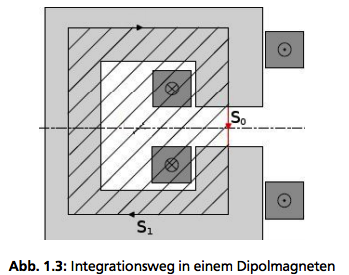
\includegraphics[width=60mm]{img/dipol.png}
\caption{C-Förmiger Dipolmagnet mit zur Bestimmung der Magnetfeldstärke verwendetem Integrationsweg \cite{anleitung}.}
\end{figure}

\subsection{Quadrupolmagnete}

Während Dipole in Beschleunigern zur Umleitung von Teilchenstrahlen verwendet werden, benutzt man Quadrupole zur Fokusierung von Strahlen. Wird ein ausgedehnter Teilchenstrahl entlang der  magnetischen Achse des Quadrupols geleitet, so wird er in einer Achsenrichtung senkrecht zum Geschwindigkeitsvektor fokusiert und in die andere Richtung defokusiert. Aus diesem Grund werdenzur Fokusierung von Teilchenstrahlen immer mehrere in Reihe geschaltete Quadrupole benötigt: Der erste Quadrupol fokusiert o.b.d.A. in x-Richtung und defokusiert in y-Richtung, während der 2. in x-Richtung defokusiert und in y-Richtung fokusiert. Da die Magnetfeldstärke und somit die auf ein bewegtes Teilchen wirkende Lorenzkraft mit zunehmendem Abstand zur magnetischen Achse zunimmt, ist bei richtiger Kalibrierung die defokusierende Wirkung des 2. Quadrupols in der x-Achse geringer als dessen fokusierende Wirkung in Richtung der y-Achse.

\begin{figure}[H]
\centering
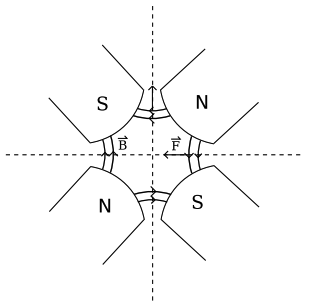
\includegraphics[width=60mm]{img/quadrupol.png}
\caption{Schematische Darstellung eines Quadrupols mit Magnetfeldlinien und Kräften, die auf ein in Zeichenebende durch den Quadrupol geleitetes negativ geladenes Teilche wirken \cite{anleitung}.}
\end{figure}

Im Idealfall sind die Polschuhe dabei von unendlich ausgedehnter, hyperbolischer Form, was sich in der Realität jedoch als unpraktikabel erweist. Aus diesem Grund werden heutzutage häufig durch numerische Näherungsverfahren für die Anwendung optimierte Polschuhe eingesetzt, um unerwünschte Dipol- oder Multipolanteile höhrer Ordnung zu unterdrücken. 

\section{Diskrete Fourier-Transformation}
Bei der Messung der Multipolkomponenten im Quadrupol kommt eine rotierende Spule zum Einsatz, wobei mit einem Oszilloskop die vom Magneten induzierte Spannung aufgenommen wird. Die so aufgenommene Spanungskurve setzt sich aus verschiedenen Sinusschwingungen zusammen, welche den jeweiligen im Quadrupol vorhandenen Multipolkomponenten entsprechen. Um diese Daten weitterzuverarbeiten, müssen zuerst die aufgneommenen Frequenzen mit Hilfer der diskreten Fourier-Transformation (DFT) isoliert werden. Vorraussetzung hierfür ist, dass die Messpunkte $x(n)$ bekannt sind und sich in konstantem zeitlichen Abstand $T$ zueinander befinden. Abgeleitet aus der Fourier-Transformation ergibt sich für die DFT:
$$X[k]= \sum_{n=0}^{N-1} x\left( n \right) \cdot \exp{-jkn \frac{2\pi}{N}}, k = 0, 1, 2, \dots, N-1$$
Mit der Anzahl der Abtastwerte N. Eine hohe Zahl für N vergrößert dabei die Feinheit der Abtastung, da das durch die DFT erhaltenen Frequenzraster k direkt von N abhängen. Die bestimmten Frequenzen ergeben sich zu 
$X[k]=k\frac{f_s}{N}$
wobei $f_s$ die Abtastfrequenz bei der Datenaufnahme angibt.

Um optimale Ergebnisse mit der DFT zu erhalten, sollte die Abtastfrequenz ein ganzzahliges Vielfache der auftretenden Schwingungsfrequenzen sein, da sie sonst durch benachtbarte Frequenzen angenähert werden müssen. Des weiteren ist darauf zu Achten, dass das aufgenommene Signal periodisch fortsetzbar ist, das Ende also möglichst sprungfrei an den Anfang anschließt. Gegebenenfalls empfiehlt es sich, Messdaten am Ende zu verwerfen, um eine möglichst gute fortsetzbarkeit zu erreichen.
\chapter{Durchführung}
\section{Vermessung des Gradientenprofils des Quadrupols}

Zuerst muss überprüft werden, ob die Achsen des Quadrupols und der zum Messen benutzten CNC-Einheit parallel zueinander sind. Dazu wird eine Messung entlang der X-Achse der CNC-Einheit aufgenommen, welche parallel zur s-Achse, also parallel zu einem potentiell durch den Quadrupol geführten Teilchenstrahl liegen sollte. Bei korrekter Positionierung des Quadrupols ist zwischen dem steilen Anstieg bzw.\ Abfall an den Rändern des Quadrupols ein Bereich konstanter Magnetfeldstärke zu erwarten.
\begin{figure}[H]
\centering
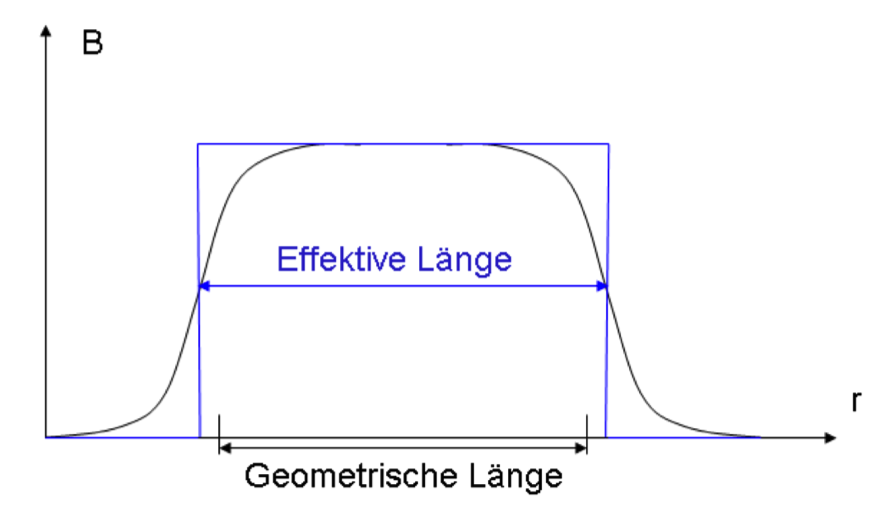
\includegraphics[width=130mm]{img/magnetfeldplateau.png}
\caption{Erwarteter Verlauf des gemessenen Magnetfeldes bei korrekter Ausrichtung des Quadrupols \cite{anleitung}}
\end{figure}
In unserem Fall war der Quadrupol bereits sehr gut ausgerichtet, im Plateau-Bereich im Inneren des Quadrupols hat sich die Magnetfeldstärke über eine Distanz von etwa $5 cm$ um weniger als $1\%$ verändert. Die Masse und unhandlichen Ausmaße des verwendete Magneten ließen es als sehr unwahrscheinlich erscheinen, durch eine manuelle Korrektur der Ausrichtung des Quadrupols eine Verbesserung zu erzielen, weswegen wir keine Veränderungen an der Ausrichtung des Magneten durchgeführt haben.

\begin{center}
\begin{figure}[H]
\begin{tikzpicture}
\begin{axis}[
    legend pos=north west,
    title={Kalibrationsmessung des Quadrupols},
    xlabel=$x$ in $mm$,
    ylabel=$B$ in $mT$,
    width=0.9\textwidth,
    height=7cm,
    xmin=0,
    xmax=225,
    grid=both,
    ymin=0,
    ymax=112,
    tick align=outside,
    tickpos=left,
    minor x tick num=3,
    minor y tick num=4,
    minor grid style={dotted,thin},
]
\addplot[red, smooth, mark=x, mark size=1pt, error bars/.cd, x dir=both, x fixed=0.25]
table[x expr=\thisrowno{0} * 5, y expr=\thisrowno{2} * (-1)] {data/Ausrichtung.txt};
\end{axis}
\end{tikzpicture}
\captionof{figure}{Gemessenes Magnetfeld für die Kalibrationsmessung in Abhängigkeit der Position der Hallsonde entlang der s- bzw.\ x-Achse im Quadrupol. Die nahezu konstante Feldstärke im Plateaubereich spricht für eine beinahe exakte Ausrichtung des Quadrupols.}
\end{figure}
\end{center}

Zur Vermessung des Quadrupols wird die Magnetfeldstärke im zuerst bei $0 A$ betriebenen Magneten mit einer Hall-Sonde an 45 Messpunkte in $5 mm$ Abständen entlang der X-Achse der CNC-Einheit aufgenommen, wobei sich sowohl die ersten als auch die letzten 6 Messpunkte außerhalb des Quadrupols befinden. Um nicht nur die Magnetfeldstärke, sondern auch ihren Gradienten bestimmen zu können, muss diese Messreihe anschließend für 5 weitere Positionen im Quadrupol in Abständen von $8mm$ entlang der Y-Achse der CNC-Einheit wiederholt werden. Diese Messreihe aus insgesamt 270 Messpunkten wurde von einem Computerprogramm nach Eingabe der gewünschten Parameter automatisch durchgeführt.

Im Anschluss wird die Messung für 5 weitere Stromstärken in Schritten von 2 A von 10 A bis 2 A wiederholt.

\section{Vermessung des Dipols in der xy-Ebene}
Analog zur Vermessung des Quadrupols wird der der "`Steerer"' Dipol vermessen. Entlang der s-Achse des Magneten bzw.\ der x-Achse der CNC-Einheit werden bei $5 A$ Betriebsstrom 51 Messpunkte im Abstand von $1 cm$ aufgenommen. Diese Messreihe wird für 11 verschiedene Positionen entlang der y-Achse mit einem Abstand von $2 mm$ automatisiert durchgeführt.

Im Gegensatz zum Quadrupol besitzt der Dipol keine abschirmende Eisenplatte an den offenen Enden des Magneten, wodurch das vom Dipol erzeugte Magnetfeld außerhalb der geometrischen Länge des Magneten deutlich langsamer abfällt. Aus diesem Grund werden jeweils 10 Magnetfeldmessungen (entsprechen $10 cm$) außerhalb des Magneten durchgeführt.

\section{Magnetfeld des Dipols in Abhängigkeit des Spulenstroms}

Um den Effekt der Hysterese auf den verwendeten Dipolmagneten zu bestimmen, wird an einer festen Position im Dipol bei Stromstärken in 1 A-Schritten von 5 A bis 0 A die Magnetfeldstärke gemessen. Bei dieser Messung ist besonders darauf zu Achten, die Stromstärke monoton auf den nächsten Messwert herunter zu regeln, da sonst durch die Eigenschaften der Hysterese die Messung verfälscht werden würde.

\section{Messung der Multipolanteile mit rotierender Spule}
Die Vermessung der Multipolanteile im Quadrupol wird mit einer rotierenden Spule im Zentrum des Magneten durchgeführt. Allerdings ergibt sich bei einer solchen Messung das Problem, dass sich durch die Symmetrie des Quadrupols in einer um ihre Symmetrieachse rotierenden Spule alle induzierten Ströme aufheben. Aus diesem Grund wurde die Messspule außermittig an die rotierende Achse des Messgerätes angebracht, was bei korrekter Ausrichtung im Quadrupol zu einer kreisförmigen Rotation der Messspule um den Mittelpol des Magneten führt.

Die zentrale Positionierung der Rotationsachse der Spule erwies sich dabei als kein triviales Unterfangen, da wir keine Möglichkeit hatten, das innere des Quadrupols und die Position der Sonde genau zu vermessen.


\chapter{Auswertung}

\section{Vermessung des Remanenzgradientenprofils des Quadrupols}
Zuerst wird das Remanenzgradientenprofil, also das Gradientenprofil des Quadrupols ohne angelegten Strom bestimmt. Dazu werden bei festgehaltenem x-Wert in y-Richtung benachbarte Messwerte des Magnetfeldes voneinander subtrahiert, was für jeden x-Wert 5 Gradienten in y-Richtung ergibt. Anschließende Mittelung über all 5 Werte und Bildung der Standardabweichung ergeben die Werte sowie die Fehler für das Gradientenprofil.
\begin{center}
\begin{figure}[H]
\begin{tikzpicture}
\begin{axis}[
    legend pos=south east,
    title={Remanenzgradientenprofil des Quadrupols},
    xlabel=$x$ in $mm$,
    ylabel=$\nabla_y (B)$ in $\frac{mT}{mm}$,
    width=0.9\textwidth,
    height=9cm,
    xmin=0,
    xmax=220,
    grid=both,
    ymin=-0.01,
    ymax=0.065,
    tick align=outside,
    tickpos=left,
    minor x tick num=3,
    minor y tick num=4,
    minor grid style={dotted,thin},
    seperators
]
\addplot[red, only marks, mark=x, mark size=1pt, error bars/.cd, x dir=both, x fixed=0.25, y dir=both, y explicit]
table[x index=0, y index=1, y error index=2] {data/parsed/m3-quad-0A-MeanGradients.txt};
\addlegendentry{Magnetfeldgradient}
\addplot[pink, mark=x, mark size=0pt, samples=20, domain=60:170] {0.0606932 + 0.0000131731*x};
\addlegendentry{Fitgerade Plateaubereich}
\addplot[teal, mark=x, mark size=0pt, samples=20, domain=20:85] {-0.0387665 + 0.00130992*x};
\addlegendentry{Fitgerade des Randfeldes}
\end{axis}
\end{tikzpicture}
\captionof{figure}{Plateauförmiges Gradientenprofil des Quadrupols, der auf Grund von Hysterese auch ohne angelegten Strom trotzdem ein Magnetfeld erzeugt. Zu sehen sind weiterhin Fitgeraden im Plateau- und Randfeld, welche Aufschluss über die Abschirmung und Ausrichtung des Quadrupolmagneten geben.}
\end{figure}
\end{center}

Der Anstieg des Magnetfeldgradienten im Randfeld des Quadrupols gibt Aufschluss darüber, wie gut der Magnet nach außen hin abgeschirmt ist. Je höher die Steigung der durch das Randfeld gefitteten Geraden, desto effektiver werden sowohl äußere als auch vom Quadrupol selbst erzeugte Magnetfelder abgeschirmt. Eine gute Abschirmung ist insbesondere beim Betrieb mehrerer Magnete in geringem Abstand wichtig, wie es zum Beispiel bei der Fokussierung von Teilchenstrahlen der Fall sein kann.



Während die Steigung der Fitgeraden durch den Gradienten des Randfeldes möglichst groß sein soll, ist bei Messung entlang der Teilchenstrahlachse eine geringe Steigung erstrebenswert. Eine betragsmäßig große Steigung im Plateaugradienten weist entweder auf einen großen Winkel zwischen Teilchenstrahlachse und magnetischer Achse des Quadrupols oder auf einen Defekt im Magneten hin.

\subsection{Fitwerte}
Sowohl im Rand- als auch im Plateaubereich des Magneten haben wir lineare Fits verwendet: 
$$f(x) = a \cdot x + b$$
Folgende Werte haben sich ergeben:

Randbereich:
\begin{center}
  \begin{tabular}{|p{2.6cm}|p{2.6cm}|p{3.5cm}|}
    \hline
    Fitparameter & Wert                   &  Standardabweichung \\ \hline
    a            & $1,31 \cdot 10^{-3}$   & $4 \cdot 10^{-5}$   \\ \hline
    b            & $-3,88 \cdot 10^{-2}$  & $2,2 \cdot 10^{-3}$ \\ \hline
	\end{tabular}
\end{center}


Plateaubereich:
\begin{center}
  \begin{tabular}{|p{2.6cm}|p{2.6cm}|p{3.5cm}|}
    \hline
    Fitparameter & Wert                  & Standardabweichung  \\ \hline
    a            & $1,31 \cdot 10^{-5}$  & $1,7 \cdot 10^{-6}$ \\ \hline
    b            & $6.07 \cdot 10^{-2}$  & $2 \cdot 10^{-4}$   \\ \hline
	\end{tabular}
\end{center}

\section{Vermessung der Gradientenprofile des Quadrupols}
Analog zum Remanenzgradientenprofils wurden die Gradientenprofile des Quadrupols für Stromstärken von $I=2A$ bis $I=10A$ vermessen und ausgewertet.
\begin{center}
\begin{figure}[H]
\begin{tikzpicture}
\begin{axis}[
    legend pos=north west,
    title={Gradientenprofile des Quadrupols},
    xlabel=$x$ in $mm$,
    ylabel=$\nabla_y (B)$ in $\frac{mT}{mm}$,
    width=0.9\textwidth,
    height=13cm,
    xmin=0,
    xmax=220,
    grid=both,
    ymin=-0.1,
    ymax=6.2,
    tick align=outside,
    tickpos=left,
    minor x tick num=3,
    minor y tick num=4,
    minor grid style={dotted,thin},
    seperators
]
\addplot[teal, only marks, mark=x, mark size=1pt, error bars/.cd, x dir=both, x fixed=0.25, y dir=both, y explicit]
table[x index=0, y index=1, y error index=2] {data/parsed/m3-quad-10A-MeanGradients.txt};
\addlegendentry{I=10A}
\addplot[orange, only marks, mark=x, mark size=1pt, error bars/.cd, x dir=both, x fixed=0.25, y dir=both, y explicit]
table[x index=0, y index=1, y error index=2] {data/parsed/m3-quad-8A-MeanGradients.txt};
\addlegendentry{I=8A}
\addplot[yellow, only marks, mark=*, mark size=1pt, error bars/.cd, x dir=both, x fixed=0.25, y dir=both, y explicit]
table[x index=0, y index=1, y error index=2] {data/parsed/m3-quad-6A-MeanGradients.txt};
\addlegendentry{I=6A}
\addplot[blue, only marks, mark=+, mark size=1pt, error bars/.cd, x dir=both, x fixed=0.25, y dir=both, y explicit]
table[x index=0, y index=1, y error index=2] {data/parsed/m3-quad-4A-MeanGradients.txt};
\addlegendentry{I=4A}
\addplot[red, only marks, mark=x, mark size=1pt, error bars/.cd, x dir=both, x fixed=0.25, y dir=both, y explicit]
table[x index=0, y index=1, y error index=2] {data/parsed/m3-quad-2A-MeanGradients.txt};
\addlegendentry{I=2A}
\end{axis}
\end{tikzpicture}
\captionof{figure}{Gradientenverlauf des Quadrupols für angelegte Stromstärken von 2A bis 10A. Bei zunehmender Stromstärke ist ein deutlicher Anstieg des Magnetfeldgradienten zu beobachten.}
\end{figure}
\end{center}

\subsection{Bestimmung der magnetischen Länge des Quadrupols}
Durch Mittelung über alle Gradientenwerte je einer Stromstärke im Plateaubereich lässt sich der maximale Gradient $g_{max}$ für diese Stromstärke bestimmen. Die Gesamtfläche unter allen Messpunkten lässt sich numerisch mit Hilfe der Trapezformel bestimmen, woraus sich die magnetische Länge des Quadrupols bestimmen lässt: $$L_m = \frac{\int_{0}^{220} g dx}{g_{max}}$$

Einsetzen der zuvor bestimmten Werte für alle von uns verwendeten Stromstärken liefert folgende Ergebnisse für die magnetische Länge des Quadrupols:
\begin{center}
  \begin{tabular}{|p{2.6cm}|p{2.6cm}|p{2.6cm}|}
    \hline
    Strom in $A$ & $L_m$ in $mm$ & $\Delta L_m$ in $mm$ \\ \hline
    0            & 123.1         & 2.2                  \\ \hline
    2            & 126.2         & 1.4                  \\ \hline
    4            & 126.2         & 1.4                  \\ \hline
    6            & 126.3         & 1.3                  \\ \hline
    8            & 126.3         & 1.4                  \\ \hline
    10           & 126.3         & 1.3                  \\ \hline
	\end{tabular}
\end{center}

Aus den einzelnen Werten der magnetischen Länge lässt sich durch Bilden des Mittelwerts ein endgültiger Wert für $L_m$ berechnen. Wir erhalten $$L_m=125,7mm\pm0,6mm$$

Dieser Wert liegt wie erwartet etwas oberhalb der geometrische Länge, welche wir auf $(120 \pm 10)mm$ abgeschätzt haben. Der relativ große Fehler von 1 cm beim Messen der geometrischen Länge liegt in der Tatsache begründet, dass sich eine Längenmessung mit Hilfe eines Zollstocks im Inneren des abgeschirmten Quadrupols selbst zu zweit als äußerst schwierig herausgestellt hat.

\section{Strom-Gradienten-Kalibrierung}
Wie schon bei Vermessung des Remanenzgradientenprofils angemerkt, erzeugt der Quadrupol auf Grund von Remanenz selbst ohne Stromzufuhr ein magnetisches Feld in seinem Inneren. Es genügt somit für den Betrieb in Beschleunigern nicht, einen unbenutzten Magneten im Teilchenstrahl einfach auszuschalten. Um im Inneren des Magneten kein Feld und somit auch keinen Magnetfeldgradienten zu erzeugen, muss ein Strom mit einer Flussrichtung entgegen der Betriebsrichtung angelegt werden.

Zur Bestimmung der Größe dieses Stroms ist es notwendig, eine Strom-Gradienten Kalibrierung durchzuführen. Dazu werden die gemessenen Plateauwerte des Magnetfeldgradienten gegen die angelegte Stromstärke aufgetragen.
\begin{center}
  \begin{tabular}{|p{2.6cm}|p{2.6cm}|p{2.6cm}|}
    \hline
    Strom in $A$ & Gradient $g$ in $mT/mm$ & $\Delta g$ in $mm$ \\ \hline
    0            & 0,062                   & 0,001              \\ \hline
    2            & 1,236                   & 0,006              \\ \hline
    4            & 2,410                   & 0,012              \\ \hline
    6            & 3,579                   & 0,016              \\ \hline
    8            & 4,738                   & 0,022              \\ \hline
    10           & 5,876                   & 0,027              \\ \hline
	\end{tabular}
\end{center}

Ein linearer Fit der Form $g(I) = m \cdot I + g_0$ erlaubt es anschließend, die Stromstärke zu bestimmen, bei der vom Quadrupol kein Magnetfeld erzeugt wird.

\begin{center}
\begin{figure}[H]
\begin{tikzpicture}
\begin{axis}[
    legend pos=south east,
    title={Strom-Gradienten-Kalibrierung des Quadrupols},
    xlabel=$I$ in $A$,
    ylabel=$\nabla_y (B)$ in $\frac{mT}{mm}$,
    width=0.9\textwidth,
    height=9cm,
    xmin=-0.5,
    xmax=10.5,
    grid=both,
    ymin=-0.2,
    ymax=6.5,
    tick align=outside,
    tickpos=left,
    minor x tick num=3,
    minor y tick num=4,
    minor grid style={dotted,thin},
    seperators
]
\addplot[red, only marks, mark=x, mark size=1pt, error bars/.cd, x dir=both, x fixed=0.02, y dir=both, y explicit]
table[x index=0, y index=1, y error index=2] {data/parsed/m3-quad-CurrentGradient.txt};
\addlegendentry{Magnetfeldgradient}
\addplot[teal, mark=x, mark size=0pt, samples=10, domain=-0.5:10.5] {0.0731429 + 0.582071*x};
\end{axis}
\end{tikzpicture}
\captionof{figure}{Der lineare Zusammenhang zwischen Magnetfeldgradient im Quadrupol und angelegter Stromstärke ist hier sehr gut zu erkennen. Die Messunsicherheiten belaufen sich bei den meisten Werten auf deutlich unter 1\% des Messwertes und sind zu geringfügig um sichtbar zu sein.}
\end{figure}
\end{center}

Wir erhalten aus dem Fit einen zum Ausschalten des Quadrupol-Magnetfeldes benötigten Strom von $$I_k=(-0,127 \pm 0.018)A$$
\subsection{Fitwerte}

Zur Strom-Gradienten-Kalibrierung wurde ein linear Fit der Form $g(I) = m \cdot I + g_0$ verwendet.
\begin{center}
  \begin{tabular}{|p{2.6cm}|p{2.6cm}|p{3.5cm}|}
    \hline
    Fitparameter & Wert    & Standardabweichung \\ \hline
    $m$          & $0,582$ & $0,002$            \\ \hline
    $g_0$        & $0,073$ & $0,010$            \\ \hline
	\end{tabular}
\end{center}

\clearpage{}
\section{Vermessung des Dipols in der xy-Ebene}

Dipole werden in Beschleunigern zum Umlenken des Teilchenstrahls verwendet. Dabei muss man jedoch darauf achten, dass das vom Teilchenstrahl passierte Feld möglichst homogen ist, da sonst der Strahl defokussiert wird. Aus diesem Grund erscheint es vernünftig, die Magnetfeldstärke im Inneren des Dipols vor der Verwendung zu vermessen.

\begin{figure}[H]
\centering
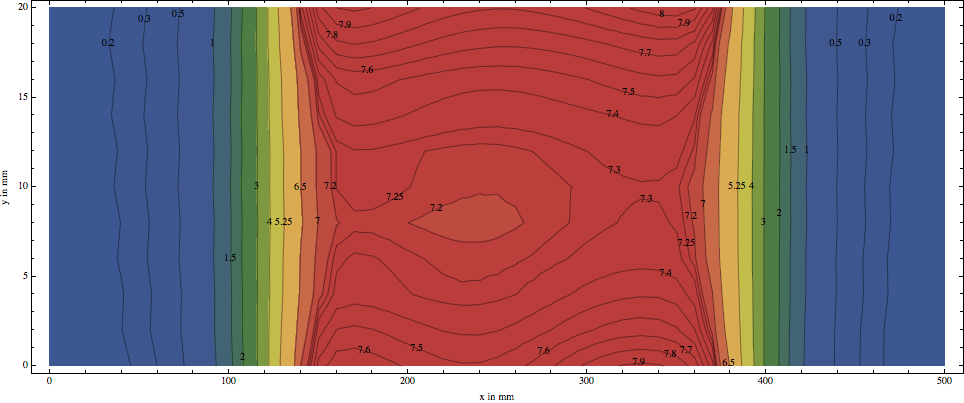
\includegraphics[width=1\textwidth]{img/steererxy.png}
\caption{Magnetfeldstärke im Steerer in Abhängigkeit von der Position. Wie erwartet ergibt sich ein starker Gradient an den offenen Enden des Steerers. Das Feld im Inneren des Steerers ist allerdings nicht wie erwartet perfekt homogen, sondern weist deutlich messbare Schwankungen auf.}
\end{figure}

Der durch das Rechteck markierte Raum ist der von uns zur Bestimmung der Magnetfeldstärke verwendete Bereich. Sowohl in x- als auch in y-Richtung treten außerhalb des Rechteckes Randeffekte auf, durch welche der Gradient des Magnetfeldes zunimmt. Durch Mittelwertbildung über alle im Rechteck befindlichen Messpunkte erhalten wir für die Magnetfeldstärke des Steerers $B=(7,229 \pm 0,074)mT$.


Bei Wahl einer Toleranz von $2\%$ als Grenze des feldglatten Bereiches erhalten wir $\Delta B=0,146mT$ und somit eine untere Schranke von $B_{min}=7,153mT$ sowie eine obere Schranke von $B_{max} = 7,445mT$. Der kleinste Wert des Magnetfeldes im Inneren des Steerers beträgt $7,173mT$ und verletzt somit nicht die Schranken des feldglatten Bereiches.

\section{Bestimung der Windungszahl des Steerers}
Der Zusammenhang zwischen Magnetfeld im Inneren einer Spule, angelegter Stromstärke und Windungszahl ist gegeben durch:

$$B = \mu_{0} \cdot I \cdot \frac{N}{L}$$

Die Höhe $L$ des Steerers haben wir mit Hilfe eines Zollstocks auf $L=(50\pm 2)mm$ bestimmt, wobei der Fehler von uns durch die nicht sehr gleichförmige Wicklung des Steerers und den damit zusammenhängenden Messschwierigkeiten mit 2 mm relativ hoch angesetzt wurde.

Der Strom des Steerers ist auf $I=(5,00 \pm 0,01)A$ eingestellt und für die Magnetfeldstärke haben wir den Mittelwert des zuvor bestimmten feldglatten Bereiches von $B=(7,299 \pm 0,0741)mT$ verwendet.

Einsetzen ergibt folgende Spulenzahl:

$$N= 58,1 \pm 2,4$$

Dies deckt sich mit dem von uns durch Abzählen der Windungen geschätzten Wert von 50 bis 60 Windungen.


\section{Messung der Multipolanteile des Quadrupols}

Im Idealfall besitzt ein Quadrupol nur eine Quadrupolkomponente. Eine Dipolkomponente oder Komponenten höherer Ordnung sind unerwünscht, treten jedoch in geringen Maßen bei den meisten Quadrupolen auf. Da der von uns benutzte Quadrupol zu einer Zeit hergestellt wurde, in dem durch numerische Optimationsverfahren optimierte Quadrupole, insbesondere die benötigten Polschuhe, nur schwer herzustellen waren, erwarten wir einen signifikanten Anteil an unerwünschten Komponenten.

Ein noch größerer Anteil unerwünschter Komponenten kommt vermutlich von der verwendeten Messmethode, insbesondere war die einzige uns zur Verfügung stehende Methode zur genauen Positionierung der rotierenden Spule unser Augenmaß. Des weiteren war aus messtechnischen Gründen die Spule außermittig an die Rotationsachse angebracht, was ein genaues Abschätzen der Positionierung weiter erschwerte. Um dies auszugleichen haben wir 3 Messungen an unterschiedlichen Positionen entlang der y-Achse durchgeführt.

\begin{center}
\begin{figure}[H]
\begin{tikzpicture}
\begin{axis}[
    legend pos=north east,
    title={Normierte Multipolanteile im Quadrupol},
    xlabel=Multipolkomponente,
    ylabel=Anteil der Multipolkomponente,
    width=0.95\textwidth,
    height=11cm,
    ybar=0pt,
    ymin=0,
    ymax=1.05,
    samples=2,
    domain=1:2,
    xtick=data,
    bar width=20,
    tick align=outside,
    tickpos=left,
    grid=both,
    minor y tick num=4,
    minor grid style={dotted,thin},
    enlarge x limits={abs=0.5},
    nodes near coords,
    every node near coord/.append style={anchor=mid west, rotate=90},
    nodes near coords align={vertical},
    seperators
]
\addplot table[x index=0, y index=1] {data/fourier/F0017CH1-Furier.txt};
\addplot table[x index=0, y index=1] {data/fourier/F0018CH1-Furier.txt};
\addplot table[x index=0, y index=1] {data/fourier/F0019CH1-Furier.txt};
\end{axis}
\end{tikzpicture}
\captionof{figure}{Gemessene Multipolkomponenten des Quadrupols, normiert auf die Quadrupolkomponente und gemessen an 3 unterschiedlichen Positionen senkrecht zur magnetischen Achse des Quadrupols.}
\end{figure}
\end{center}

Während die Multipolkomponenten höherer Ordnung bei allen 3 Messungen annähernd gleich ausfielen, ist eine deutliche geringere Dipolkomponente bei der ersten Messung zu sehen, was auf eine zentralere Positionierung der rotierenden Spule schließend lässt. Dennoch ist die Dipolkomponente mit 21\% des Quadrupolanteils sehr groß.

Sogar die höheren Multipolkomponenten, welche im Vergleich zur Dipolkomponente klein ausfallen, liegen deutlich über den für Teilchenbeschleunigern erwünschten Toleranzgrenzen, welche im Promille- bis geringen Prozentbreich liegen.


\chapter{Fazit}
Im diesem Versuch ist es uns gelungen, einen Quadrupolmagneten sowohl im Bezug auf sein Gradientenprofil als auch auf seine Multipolkomponenten zu vermessen. Die Vermessung des Gradientenprofils war auf Grund der verwendeten Messaparatur sehr genau möglich, was es uns ermöglicht hat, die magnetische Länge des Quadrupols mit geringer Messunsicherheit von weniger als 0.5\$ anzugeben. Die Vermessung der Multipolkomponenten hat sich als schwieriger erwiesen, da für uns eine exakte Positionierung der rotierenden Spule im Inneren des Quadrupols nicht möglich war. Dies haben wir durch wiederholte Messungen an leicht unterschiedlichen Positionen versucht auszugleichen.

Weiterhin konnten wir eine genaue Vermessung des Magnetfeldes in einer Ebene im Inneren des Dipols durchführen. Dabei haben wir festgestellt, dass das vom Dipol erzeugte Feld keinesfalls homogen ist, sondern deutliche Unregelmäßigkeiten aufweist. Dies stammt möglicherweise von der nicht genauen Wicklung des Spulendrahtes.

%ENDE INHALT
\cleardoublepage{}
% Eintrag fürs Inhaltsverzeichnis
\newpage
\begin{thebibliography}{100}
  \bibitem{anleitung} \url{Versuchsanleitung}
  \bibitem{hysterese} \url{http://www.chemgapedia.de/vsengine/media/vsc/de/ph/14/ep/einfuehrung/magnetfeld/bilder/hysterese.png}
\end{thebibliography}
\end{document}
